Bei den Laufzeitmessungen des Programms wurde eine Matrize mit den Dimensionen $8192 \times 8192$ verwendet. Diese Matrix wurde mit Hilfe des \texttt{pixelpattern}-Generators erstellt und enthielt $321413$ Komponenten, die im Schnitt $87.5$ Pixel groß waren (der Generator wird näher bei \ref{pixelpattern} auf Seite \pageref{pixelpattern} beschrieben).

Bei den Messungen wurde das Programm jeweils mit $1$, $2$, $4$ und $8$ Prozessoren ausgeführt. Für jede Anzahl der Prozessoren wurden $10$ Programmdurchläufe gemacht, um Schwankungen auszuschließen (wie man in den Messergebnissen sehen kann, waren die Schwankungen nicht sehr groß).

\subsection{Gesamtlaufzeit} \label{bench:whole}

In Abbildung \ref{fig:bench_whole} auf Seite \pageref{fig:bench_whole} sind die Gesamtlaufzeiten für die gemessenen Prozessor-Kombinationen zu sehen.

\begin{figure}[tbhp]
	\centering
	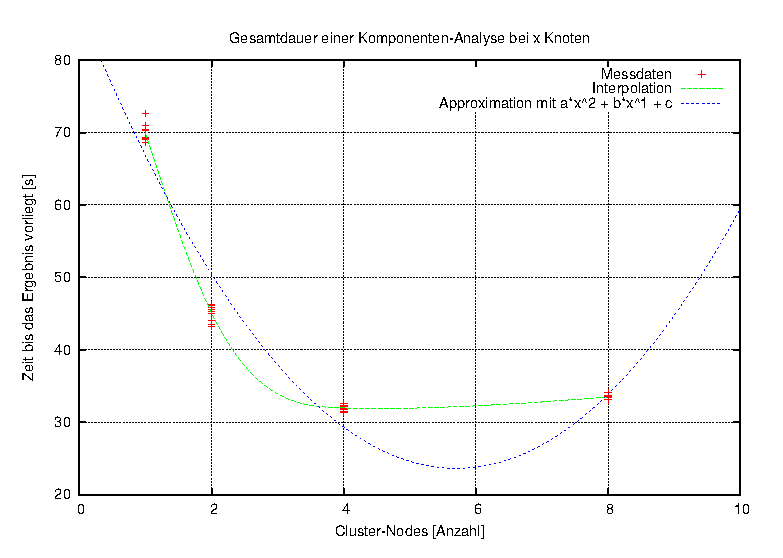
\includegraphics[width=0.9\textwidth]{images/whole_plod.eps}
	\caption{Messung der Gesamtlaufzeit}
	\label{fig:bench_whole}
\end{figure}

Wie man sieht, nimmt die Laufzeit bis zu einer Cluster-Größe von 4 Prozessoren stetig ab, um dann bei einer Größe von 8 wieder anzusteigen. Die angegeben Interpolation der Messwerte gibt dabei die Laufzeit besser wieder, als die Approximation (bei einer weiteren Testmessung mit 6 Prozessoren wurde keine wesentliche Verbesserung zu 4 Prozessoren festgestellt).

\subsection{Laufzeiten der Einzel-Aufgaben} \label{bench:task}

Warum die Gesamtlaufzeit bei 8 Prozessoren wieder steigt ist in Abbildung \ref{fig:bench_tasks} auf Seite \pageref{fig:bench_tasks} gut zu sehen. Hier werden jeweils die Laufzeiten der einzelnen Aufgaben dargestellt.

\begin{figure}[tbhp]
	\centering
	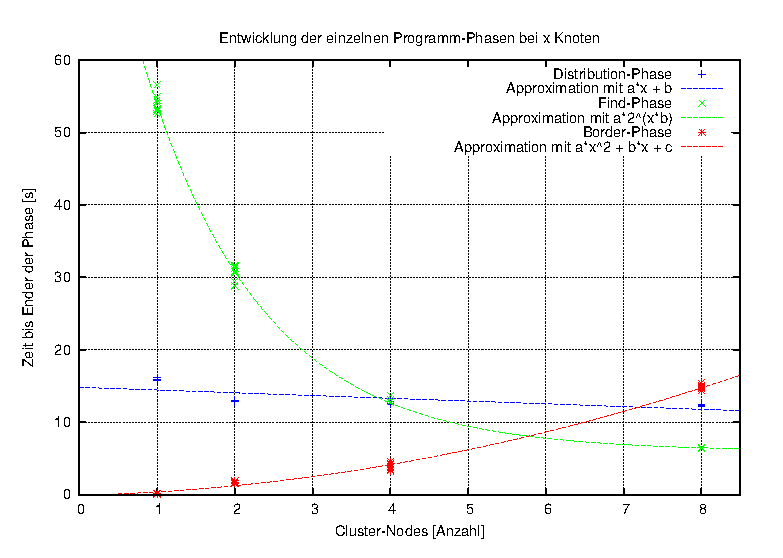
\includegraphics[width=0.9\textwidth]{images/phases.eps}
	\caption{Messung der Laufzeit der einzelnen Aufgaben}
	\label{fig:bench_tasks}
\end{figure}

Zu sehen ist, dass die Verteilung der Matrix im wesentliche gleich bleibt, die Laufzeit dieser Phase ist wesentlich durch das Einlesen der Matrix vom Dateisystem und der Geschwindigkeit des Netzwerks zur Übertragung beschränkt. Insgesamt müssen $192MByte$ von der Festplatte gelesen werde und ca. $48MByte$ übertragen werden (die genaue Größe bei der Übertragung hängt natürlich von der Größe des Clusters ab, da dann die Matrizen anders dimensioniert werden).

Was auch gut zu sehen ist, ist das lineare Laufzeitverhalten der lokalen Erkennungsphase, halbiert sich die Größe der lokalen Matrix, halbiert sich auch die Laufzeit der Erkennungsphase.

Schließlich übersteigen die Kosten der letzten Programm-Phase aber die, der Einsparung in der Erkennungsphase. Der Grund dafür ist offensichtlich. Je größer der Cluster wird, desto öfter müssen Ränder abgeglichen werden und desto länger muss der letzte Prozess warten, bis er das Ergebnis vorliegen hat. Außerdem steigt die Anzahl der übermittelten Komponenten bei jedem Prozessor an (begründet durch die hohe Anzahl in der Test-Matrix), dadurch steigt der Aufwand im Abgleich der Komponenten.